\documentclass{article}
\usepackage{tikz}
\usetikzlibrary{arrows.meta}

\begin{document}

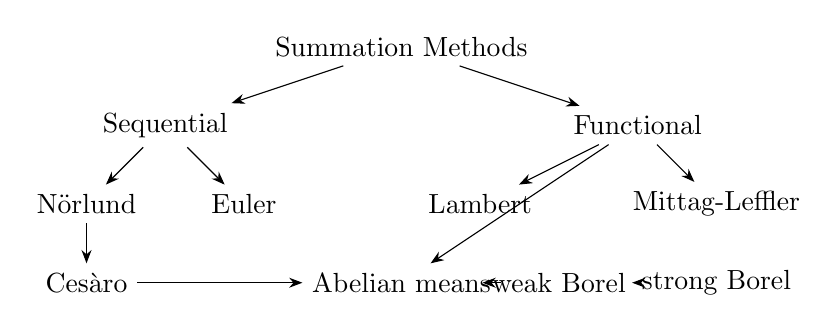
\begin{tikzpicture}[>=Stealth]

\node (summation) at (3,4) {Summation Methods};

\node (sequential) at (0,3) {Sequential};
\node (functional) at (6,3) {Functional};

\node (norlund) at (-1,2) {Nörlund};
\node (euler) at (1,2) {Euler};

\node (cesaro) at (-1,1) {Cesàro};
\node (abel) at (3,1) {Abelian means};

\node (lambert) at (4,2) {Lambert};
\node (mittag) at (7,2) {Mittag-Leffler};

\node (weakborel) at (5,1) {weak Borel};
\node (strongborel) at (7,1) {strong Borel};

\draw[->] (summation) -- (sequential);
\draw[->] (summation) -- (functional);

\draw[->] (sequential) -- (norlund);
\draw[->] (sequential) -- (euler);

\draw[->] (norlund) -- (cesaro);
\draw[->] (cesaro) -- (abel);

\draw[->] (functional) -- (abel);
\draw[->] (functional) -- (lambert);
\draw[->] (functional) -- (mittag);

\draw[->] (abel) -- (weakborel);
\draw[->] (weakborel) -- (strongborel);

\end{tikzpicture}

\end{document}